Para melhorar os problemas de convergência do método de Newton, foram feitas algumas alterações, como diminuir o avanço em uma dada direção $ d^k $, da forma:

\begin{equation}
	x^{k+1} = x^k + \alpha_k d^k
\end{equation}

onde $ \alpha_k $ minimiza $ \tilde{f}(\alpha) = f(x^k + \alpha d^k) $.

O problema resultante do sinal negativo da hessiana pode ser desviado usando um truque matricial segundo a equação \ref{eq:newton_mod_hess}. 

\begin{equation}
	F^k = G^k + \gamma I_n
	\label{eq:newton_mod_hess}
\end{equation}

Sendo $ I_n $ a matriz identidade de ordem n, é sempre possível encontrar $ \gamma $ tal que $ F_k $ tenha seus autovalores positivos e possa, assim, ser usada para gerar uma direção $ d^k $ que seja realmente de descida.
Em que $ F^k $ tem autovalores positivos para poder gerar uma direção $ d^k $ de descida segundo a equação \ref{eq:newton_mod_dk}.

\begin{equation}
	d^k = -[F^k]^{-1}g^k = -[\nabla^2 f(x^k) + \gamma I_n]^{-1}\nabla f(x^k)
	\label{eq:newton_mod_dk}
\end{equation}

Depois de construído o algoritmo, foram testadas quatro funções para efeitos de comparação:

\begin{itemize}
	\item $ f_1(x,y) = x^2 + y^2$
	\item $ f_2(x,y) = -e^{-x^2 -y^2}$
	\item $ f_3(x,y) = cos(\frac{xy}{5})+sin(\frac{xy}{5}) $
	\item $ f_4(x,y) = |x+y| $
\end{itemize}

\newpage


\begin{figure}[H]
	\begin{center}
		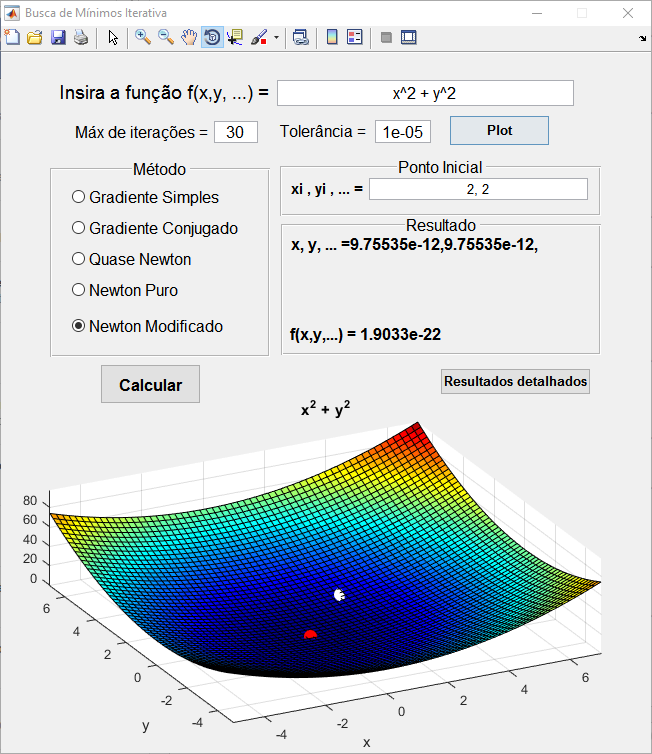
\includegraphics[width=12cm]{../newton_mod/f1_gui}   
		\caption{Janela de inicialização de $ f_1(x,y) $}
		\label{fig:newton_mod_f1_gui}
	\end{center}
\end{figure}

\begin{figure}[H]
	\begin{center}
		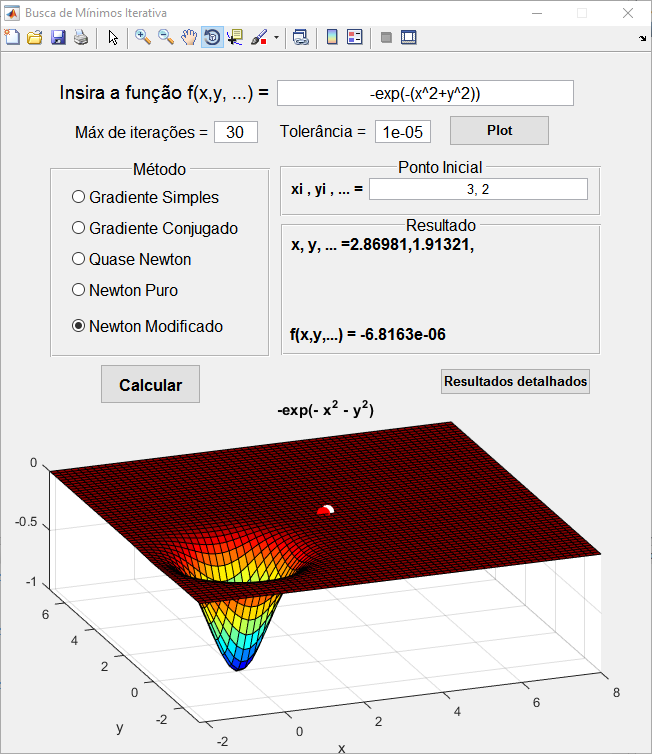
\includegraphics[width=12cm]{../newton_mod/f2_gui}   
		\caption{Janela de inicialização de $ f_2(x,y) $}
		\label{fig:newton_mod_f2_gui}
	\end{center}
\end{figure}

\begin{figure}[H]
	\begin{center}
		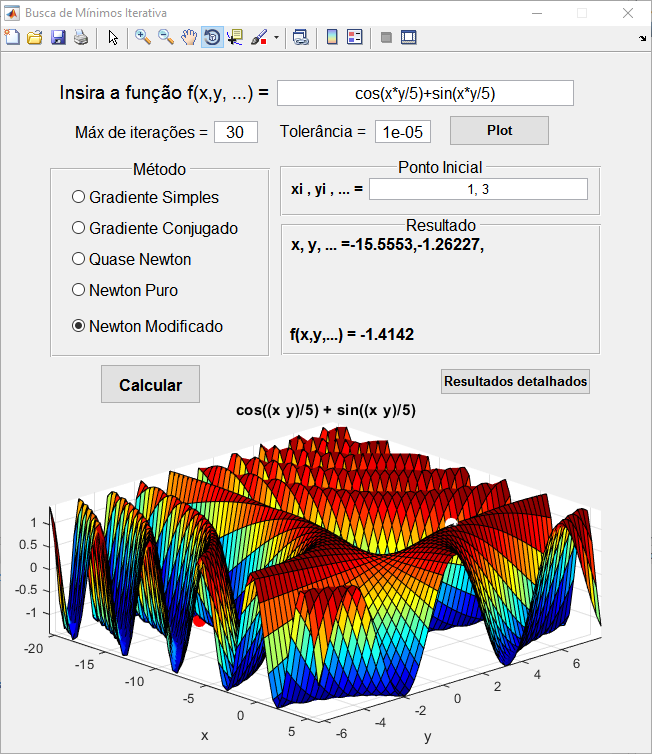
\includegraphics[width=12cm]{../newton_mod/f3_gui}   
		\caption{Janela de inicialização de $ f_3(x,y) $}
		\label{fig:newton_mod_f3_gui}
	\end{center}
\end{figure}

\begin{figure}[H]
	\begin{center}
		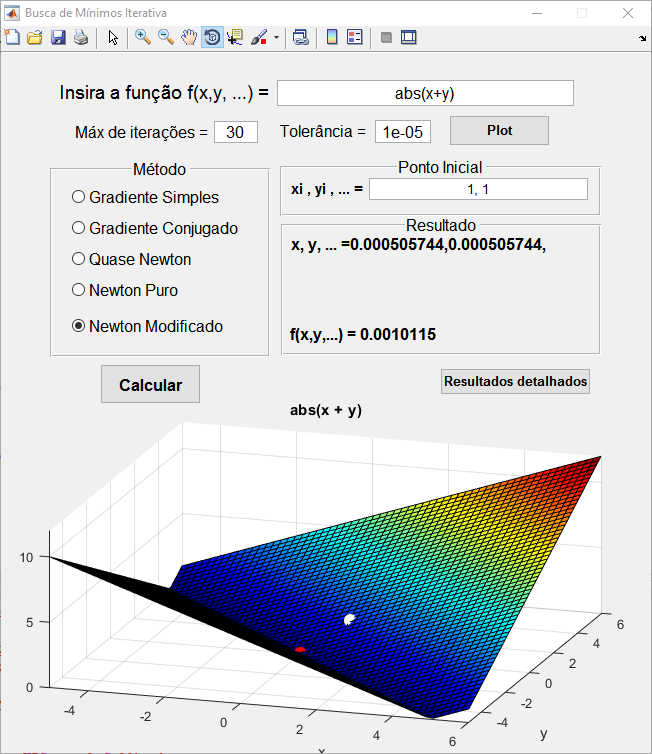
\includegraphics[width=12cm]{../newton_mod/f4_gui}   
		\caption{Janela de inicialização de $ f_4(x,y) $}
		\label{fig:newton_mod_f4_gui}
	\end{center}
\end{figure}
